\documentclass[a4paper,oneside,12pt]{book}
\def \code#1{\texttt{#1}}
\usepackage[utf8]{inputenc}
\usepackage[italian]{babel}
\usepackage[T1]{fontenc}
\usepackage{geometry}
\usepackage{graphicx}
\usepackage{placeins}
\usepackage{siunitx}
\usepackage{tikz}
\usepackage{blindtext}
\usepackage{enumitem}
\usepackage{caption}

\usepackage{booktabs}
\usepackage{array}
\usepackage{makecell}
\usepackage{float}
\usepackage{amsmath}
\usetikzlibrary{calc}
\restylefloat{table}

\newcommand*{\GridSize}{10}


\newcommand*{\TextColumnTen}[3]{% #1 = list of x/y\text
\foreach \x/\y/\text in {#1} {
\node [draw=none, thick]
at (\x-.5,#2+0.5-\y) {\text};
}%
}%
\newcommand*{\ColorCellsTen}[3]{% #1 = list of x/y/color
\foreach \x/\y/\color in {#1} {
\node [fill=\color, draw=none, thick, minimum size=#3]
at (\x-.5,#2+0.5-\y) {};
}%
}%

\newcommand*{\ColorCellsBlackTen}[3]{% #1 = list of x/y/color
\foreach \x/\y in {#1} {
\node [fill=black, draw=none, thick, minimum size=#3]
at (\x-.5,#2+0.5-\y) {};
}%
}%

\begin{document}
    \newgeometry{textwidth=15cm}
    \begin{center}
    {\LARGE {\bf Intelligenza Artificiale e Laboratorio}\\
    \vspace*{6mm}}
    {\Large Anno Accademico 2017/18}\\
    \vspace*{6mm}
    \vspace*{6mm}
    Liccardo Francesco, Mittone Gianluca, Scaletta Marco
    \end{center}
    \pagenumbering{gobble}
    %-- checked
    \newpage
    \chapter*{Programmazione Prolog e ASP}
    \section*{Implementazione di strategie di ricerca con Prolog}
    Tutti gli algoritmi di seguito descritti sono stati realizzati cercando di rendere il codice il più 	leggibile e semplice possibile: questo ha portato alla creazione di strutture molto modulari, 	formate da regole piccole, chiare e ben specializzate. Tale approccio si è rivelato 	determinante nelle fasi di debugging, testing e aggiornamento del codice semplificando e 	riducendo di molto i tempi e la quantità di lavoro richiesta per le suddette operazioni, 	aumentando però la verbosità generale dell’implementazione.

    Si è inoltre scelto di limitare l’output degli algoritmi solamente al primo risultato, 	dato che è garantito essere ottimo. A livello implementativo tale politica è stata realizzata 	mediante l’eliminazione dei punti di scelta del backtracking considerati superflui, attraverso l’uso del 	\textit{cut}.
    \subsection*{Strategie non informate}
    \subsubsection{Iterative Deepening}

    L’implementazione dell’algoritmo risulta semplice e naturale grazie al meccanismo di backtracking offerto da Prolog. Alla base vi è una ricerca a profondità limitata standard: nel caso lo stato in esame risulti finale la regola termina con successo, altrimenti viene esplorato uno stato successivo se esso non supera il livello di taglio. Esplorare uno stato significa generare una azione valida per esso, applicarla, controllare di non aver scoperto una configurazione già precedentemente analizzata ed, in tal caso, ripetere il procedimento dall’inizio. Tale algoritmo è denominato
    \code{ricerca\_profondita\_limitata} e viene eseguito ripetutamente aumentando il livello di taglio nel caso si superi tale valore senza che venga trovata una soluzione; questa ciclicità viene gestita dalla regola \code{ricerca\_profondita\_iterativa}.

    L’inizializzazione dello stato iniziale e del livello di taglio sono invece delegate a \code{iterativeDeepening}, che è la regola da richiamare per avviare la ricerca:

    \begin{center}
        \code{iterativeDeepening(Soluzione)}
    \end{center}
    dove \code{Soluzione} è la variabile che conterrà l’eventuale risultato.

    La sequenza di azioni che conducono dallo stato iniziale a quello finale viene 		elaborata mediante una strategia backward: una volta raggiunto un obiettivo la lista 		soluzione viene costruita percorrendo a ritroso il ramo che ha portato al goal, 			aggiungendo in testa alla lista tutte le azioni che vengono trovate durante il cammino.

    \subsection*{Strategie basate su euristica}
    \subsubsection{Algoritmo A*}
    Essendo questo algoritmo più complesso rispetto al precedente, si rende necessaria la creazione di una struttura dati ad hoc per associare ad un determinato stato del problema tutte le informazioni ad esso correlate. Si definisce così un nodo:
    \begin{center}
        \code{nodo(Stato, DistanzaInizio, StimaEuristica, StimaTotale, Percorso)}
    \end{center}
    dove:
    \begin{itemize}
        \item \code{Stato}: è uno stato proprio del dominio del problema;
        \item \code{DistanzaInizio}: è la distanza di Stato dallo stato iniziale;
        \item \code{StimaEuristica}: è la distanza stimata da Stato allo stato finale;
        \item \code{StimaTotale}: è la somma di \code{DistanzaInizio} e \code{StimaEuristica};
        \item \code{Percorso}: è la lista delle azioni che hanno portato a \code{Stato} dallo stato iniziale.
    \end{itemize}
    Per avviare la ricerca è sufficiente digitare
    \begin{center}
        \code{aStar(Soluzione)}
    \end{center}
    con \code{Soluzione} variabile che conterrà l’eventuale soluzione del problema. Questa regola inizializza lo stato iniziale, calcola la stima euristica della sua distanza dallo stato finale, inserisce tutte queste informazioni in un nodo e richiama \code{esplora}, che implementa 'ad alto livello' il cuore di \code{aStar}. Formalmente:
    \begin{center}

        \code{esplora(Frontiera, NodiEsplorati, Soluzione)}
    \end{center}


    dove:
    \begin{itemize}
        \item \code{Frontiera} (o open set): la lista di nodi da essere valutati;
        \item \code{NodiEsplorati} (o close set): la lista di nodi già valutati;
        \item \code{Soluzione}: lista di mosse che hanno portano allo stato finale.
    \end{itemize}

    Il primo passo ad essere eseguito è il controllo della corrispondenza tra lo stato con il valore minimo di \code{StimaTotale} (quindi il più promettente per A*) e uno stato finale. In caso positivo l’esecuzione termina e viene restituito all’utente il campo \code{Percorso} del nodo in oggetto; altrimenti si procede alla generazione di tutti i suoi successori ed alla loro analisi, con conseguente aggiornamento della \code{Frontiera}, per poi ripetere esplora ricorsivamente.

    La generazione dei successori utilizza il predicato \code{findall} per ottenere la lista completa delle azioni valide nello stato esaminato. Viene generato un nodo per ognuno dei possibili stati risultato dell’applicazione delle stesse e ne vengono compilati tutti i campi.

    Ora la regola \code{analizza} si occuperà di implementare il principio della ‘disuguaglianza triangolare’: esaminerà ogni singolo nodo successore appena generato e in base a \code{Stato} e \code{StimaTotale} deciderà se debba essere inserito in \code{Frontiera}, \code{NodiEsplorati} o se non vada considerato. L’inserimento di un nodo in \code{Frontiera} avviene sempre in modo ordinato: il primo nodo della lista sarà sempre quello con il valore minimo di \code{StimaTotale}, semplificando così le operazioni di \code{esplora}. L’esecuzione ricomincia quindi dal controllo dello stato finale.

    La scelta di adottare una struttura dati così completa per formalizzare un nodo ha il pregio di dover eseguire molti calcoli solamente una volta nella storia dello stesso, permettendo di realizzare delle regole ben specializzate e semplici, andando però ad appesantire la quantità di informazioni che l’algoritmo deve memorizzare e trasmettere da una regola all’altra.

    \subsubsection{Algoritmo IDA*}
    Questo algoritmo riutilizza la struttura \code{nodo} descritta precedentemente per associare ad un determinato stato del problema tutte le informazione ad esso correlate.
    Per avviare la ricerca è sufficiente digitare
    \begin{center}
        \code{idaStar(Soluzione)}
    \end{center}
    come primo passo controlla se vi è la presenza di un limite soglia di un'esecuzione precedente dell'algoritmo. Successivamente, indipendentemente dal passo precedente, inizializza lo stato iniziale, calcola la stima euristica della sua distanza dallo stato finale, asserisce il limite soglia inizializzandolo con il valore \code{StimaEuristica} dello stato iniziale e infine chiama la regola \code{idaStarR}.
    Formalmente:
    \begin{center}
        \code{idaStarR(Stato, StimaEuristica, Soluzione)}
    \end{center}
    dove:
    \begin{itemize}
        \item \code{Stato}: è uno stato proprio del dominio del problema;
        \item \code{StimaEuristica}: stima euristica del nodo;
        \item \code{Soluzione}: variabile che conterrà il percorso della soluzione.
    \end{itemize}

    All'interno del corpo della regola recupera l'informazione relativa al limite soglia, memorizzandola all'interno della variabile \code{Limite}, in seguito rimuove l'informazione per inizializzarla nuovamente al valore infinito (nel nostro caso a 99999, in quanto prolog non prevede una costante che identifica un valore che allegoricamente rappresenta l'infinito). Dopo aver eseguito questa sequenza di istruzioni, l'algoritmo invoca la regola \code{esplora} che rappresenta il "cuore" del processo. Formalmente:
    \begin{center}

        \code{esplora(Nodo, NodiEsplorati, Limite, Soluzione)}
    \end{center}
    dove:
    \begin{itemize}
        \item \code{Nodo}: nodo da controllare;
        \item \code{NodiEsplorati}: la lista di nodi già valutati;
        \item \code{Limite}: limite soglia dell'attuale iterazione;
        \item \code{Soluzione}: lista di mosse che hanno portano allo stato finale.
    \end{itemize}
    Come primo passo controlla se la \code{StimaTotale} del nodo è minore o uguale del limite soglia, in caso positivo effettua un'ulteriore analisi che controlla se il nodo che sta analizzando è un nodo obiettivo. Se quest'ultimo test viene superato l'algoritmo termina e viene restituito all'utente il campo \code{Percorso} del nodo in oggetto; altrimenti si procede alla generazione del nodo successore, per poi ripetere l'esplora ricorsivamente. \\
    Nel caso in cui nel primo passo la \code{StimaTotale} è maggiore del limite soglia viene controllato il valore soglia della prossima iterazione, chiamando la regola \code{verifica\textunderscore limite}. Formalmente:

    \begin{center}

        \code{verifica\textunderscore limite(StimaTotale)}
    \end{center}
    dove:
    \begin{itemize}
        \item \code{StimaTotale}: stima totale del nodo che ha superato il limite soglia dell'esecuzione.
    \end{itemize}
    Innanzitutto recupera il valore soglia della prossima iterazione e lo memorizza nella variabile \code{ProssimoLimite}, successivamente verifica se quest'ultimo è minore o uguale della \code{StimaTotale}. In caso positivo il valore del prossimo limite soglia non verrà modificato, invece in caso negativo il valore limite della prossima iterazione viene inizializzato a \code{StimaTotale}. \\
    Si ricorda che all'interno del prossimo valore soglia dovrà sempre esserci il valore minore fra tutte le stime dei costi dei nodi che hanno superato il valore soglia durante iterazione. \\
    L'implementazione dell'algoritmo è stata possibile sfruttando i due predicati \code{assert} e \code{retract} che hanno l'effetto di modificare l'insieme delle clausole del programma (alla successiva invocazione del goal). Nel caso specifico di fallimento dovuto al superamento del valore soglia è stato possibile salvare (con \code{assert}) il valore della stima totale del costo del nodo prima di fare backtracking.

    \subsubsection{Domini}
    Prima di discutere i risultati dei test degli algoritmi implementati si rende necessario esplicitare su quali domini essi siano stati messi alla prova e di come essi siano stati modellati. Ai fini di questa relazione sono stati analizzati due modelli di dominio: il \textit{labirinto} ed il \textit{gioco dell’8}, entrambi in quattro varianti caratterizzati da livelli di difficoltà diversi.

    Il \textit{labirinto} è stato modellato attraverso dei fatti che ne descrivono il numero di righe, di colonne, le caselle occupate, la posizione di partenza e quella di arrivo. Una posizione è denotata da \code{pos(Riga, Colonna)} dove i parametri sono autoesplicativi. Sono rese disponibili due possibili scenari: uno da 10x10 caselle ed uno da 20x20, ed ognuno di essi con due disposizioni delle posizioni di partenza ed arrivo, una semplice ed una difficile.


    Il gioco dell’8 invece mette a disposizione solo tre fatti: la configurazione di partenza, quella di arrivo ed il lato della griglia di gioco. Una posizione viene rappresentata mediante una lista che elenca il numero delle tessere da destra verso sinistra, dall’alto verso il basso, con una x nella posizione vuota. Anche questo dominio è stato realizzato in due varianti: una con una griglia 3x3 (gioco dell’8) ed una con una griglia 4x4 (gioco del 15), entrambe con due posizioni di partenza, una semplice ed una difficile.

    Ogni dominio è inoltre affiancato da un file contenente le relative azioni, che sono sempre quattro:

    \begin{itemize}
        \item \code{applicabile(Azione, Posizione)}: determina la validità di Azione in Posizione;
        \item \code{trasforma(Azione, Posizione, NuovaPosizione)}: applica Azione a Posizione;
        \item euristica(Posizione, StimaEuristica): calcola la stima euristica da Posizione alla posizione finale;
        \item \code{costoSpostamento(PosizionePartenza, PosizioneArrivo, Costo)}: calcola il costo di spostamento da PosizionePartenza a PosizioneArrivo.
    \end{itemize}
    In tutti i test come funzione euristica è stata utilizzata la \textit{Distanza di Manhattan} ed il costo di spostamento, data la tipologia di domini, è stato considerato unitario.

    Tutte le prove effettuate hanno confermato una netta superiorità di \textit{IDA*} rispetto agli altri algoritmi, in tutti i possibili scenari. Solo \textit{A*} riesce parzialmente a competere con esso, non riuscendo tuttavia a risolvere in tempi ragionevoli il gioco del 15 partendo dalla posizione difficile. Si dimostra invece una completa incapacità di \textit{iterative deepening} di risolvere qualsiasi problema che sia poco più che basilare: i suoi tempi di esecuzione salgono troppo rapidamente ed il numero di inferenze eseguite anche. Il caso più evidente di questo è sicuramente il test del 3x3 difficile: \textit{iterative deepening} arriva a toccare le 1.061.310.227 inferenze in 122,934 secondi, contro le 18.345.153 in 2,477 si \textit{A*} e le 623.902 in 0,076 di \textit{IDA*}. Nota a margine, \textit{A*} riesce a comportarsi meglio di \textit{IDA*} fintantoché lo scenario rimane semplice, questo per via della sua logica più semplice ed intuitiva, ma appena la complessità aumenta non è più neanche paragonabile.

    Seguono, nelle prossime pagine, grafici e tabelle riassuntive dei test condotti.
    \newgeometry{top=0.3in,bottom=0.3in,textwidth=20cm}

    \begin{center}
        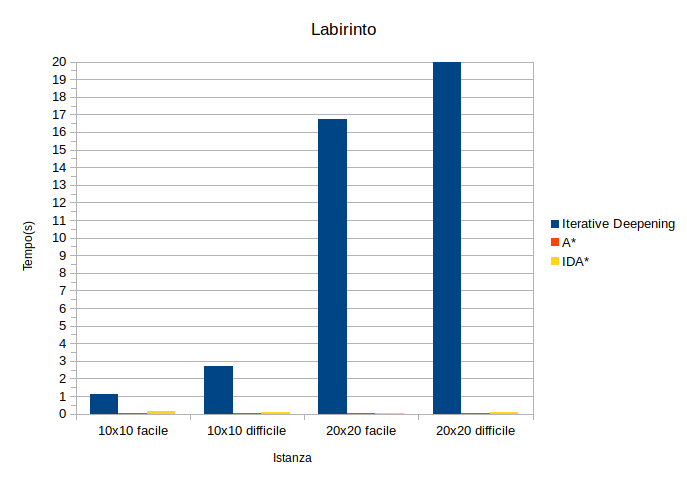
\includegraphics[height=0.70\textwidth	]{labirintoTempo}
        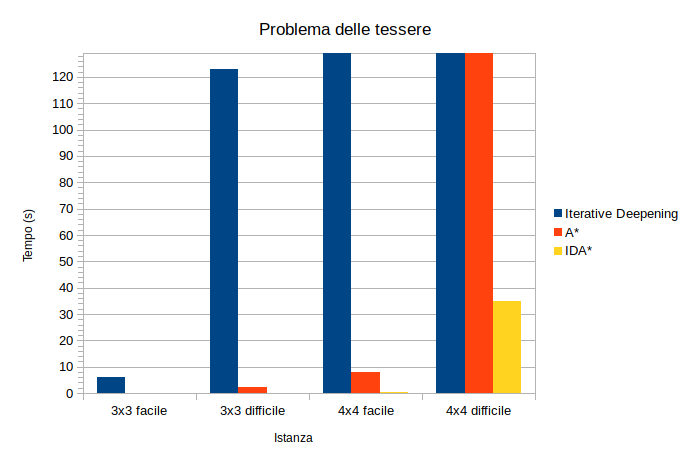
\includegraphics[height=0.70\textwidth]{tessereTempo}
        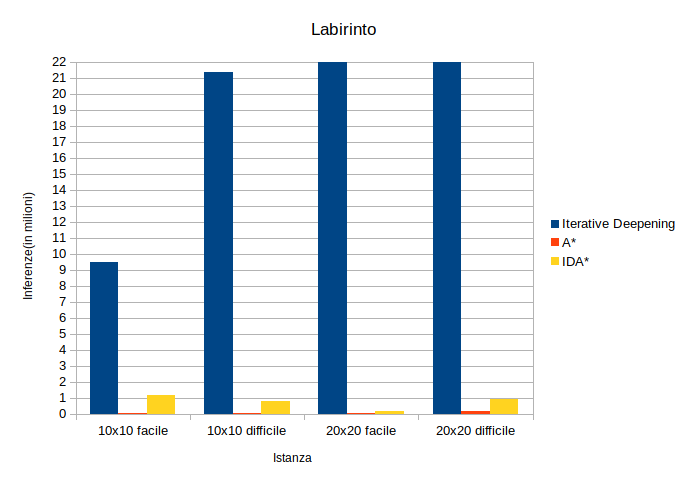
\includegraphics[height=0.70\textwidth]{labirintoInferenze}

        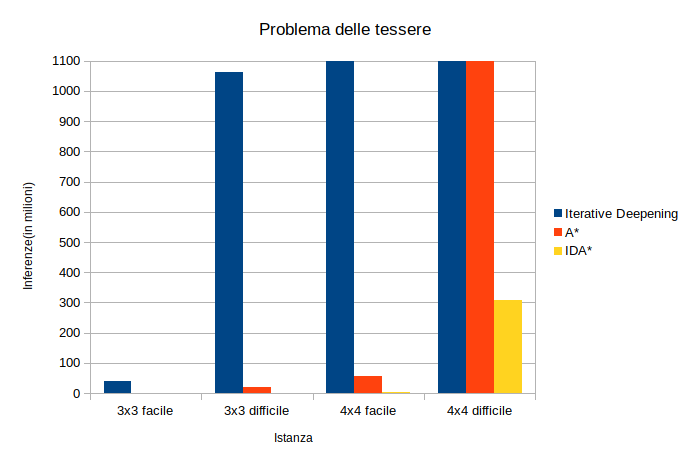
\includegraphics[height=0.65\textwidth]{tessereInferenze}

        \restoregeometry
        \newpage
        \restoregeometry
    \end{center}

    \begin{table}
        \centering
        \begin{tabular}{l c c c c}
            \toprule % Top horizontal line
            & \multicolumn{4}{c}{Labirinto} \\ % Amalgamating several columns into one cell is done using the \multicolumn command as seen on this line
            \cmidrule(l){2-5} % Horizontal line spanning less than the full width of the table - you can add (r) or (l) just before the opening curly bracket to shorten the rule on the left or right side
            Strategia & 10x10 facile & 10x10 difficile & 20x20 facile & 20x20 difficile\\ % Column names row
            \midrule % In-table horizontal line
            Iterative Deepening & 1.085 & 2.721 & 16.721 & --- \\ % Content row 1
            A* & 0.014 & 0.007 & 0.009 & 0.026\\ % Content row 2
            IDA* & 0.129 & 0.088 & 0.028 & 0.104 \\ % Content row 3

            \bottomrule
        \end{tabular}
        \caption{Tempi di esecuzione (espressi in secondi)}
    \end{table}
    \begin{table}
        \centering
        \begin{tabular}{l c c c c}
            \toprule % Top horizontal line
            & \multicolumn{4}{c}{Tessere} \\ % Amalgamating several columns into one cell is done using the \multicolumn command as seen on this line
            \cmidrule(l){2-5} % Horizontal line spanning less than the full width of the table - you can add (r) or (l) just before the opening curly bracket to shorten the rule on the left or right side
            Strategia & 3x3 facile & 3x3 difficile & 4x4 facile & 4x4 difficile\\ % Column names row
            \midrule % In-table horizontal line
            Iterative Deepening
            & 6.152	 & 122.934 & --- & --- \\ % Content row 1
            A*
            & 0.137 & 2.477 & 8.040 & ---\\ % Content row 2
            IDA*
            & 0.017 & 0.076 & 0.237 & 34.913 \\ % Content row 3

            \bottomrule
        \end{tabular}
        \caption{Tempi di esecuzione (espressi in secondi)}
    \end{table}
    \begin{table}
        \centering
        \begin{tabular}{l c c c c}
            \toprule % Top horizontal line
            & \multicolumn{4}{c}{Labirinto} \\ % Amalgamating several columns into one cell is done using the \multicolumn command as seen on this line
            \cmidrule(l){2-5} % Horizontal line spanning less than the full width of the table - you can add (r) or (l) just before the opening curly bracket to shorten the rule on the left or right side
            Strategia & 10x10 facile & 10x10 difficile & 20x20 facile & 20x20 difficile\\ % Column names row
            \midrule % In-table horizontal line
            Iterative Deepening
            & \num{9449000}& \num{21322628} & \num{141789264} & --- \\ % Content row 1
            A*
            & \num{31283} & \num{56044} & \num{27841} & \num{135345}\\ % Content row 2
            IDA*
            & \num{1189329} & \num{798983} & \num{192960} & \num{902824} \\ % Content row 3

            \bottomrule
        \end{tabular}
        \caption{Inferenze eseguite}
    \end{table}
    \begin{table}
        \centering
        \begin{tabular}{l c c c c}
            \toprule % Top horizontal line
            & \multicolumn{4}{c}{Tessere} \\ % Amalgamating several columns into one cell is done using the \multicolumn command as seen on this line
            \cmidrule(l){2-5} % Horizontal line spanning less than the full width of the table - you can add (r) or (l) just before the opening curly bracket to shorten the rule on the left or right side
            Strategia & 3x3 facile & 3x3 difficile & 4x4 facile & 4x4 difficile\\ % Column names row
            \midrule % In-table horizontal line
            Iterative Deepening
            & \num{39220382}& \num{1061310227} & --- & --- \\ % Content row 1
            A*
            & \num{682069} & \num{18345153} & \num{54955687	} & --- \\ % Content row 2
            IDA*
            & \num{138358} & \num{623902} & \num{1876229} & \num{306883838}\\ % Content row 3
            \bottomrule
        \end{tabular}
        \caption{Inferenze eseguite}
    \end{table}
    \FloatBarrier
    \restoregeometry
    \section*{Constraint Satisfaction Problem con ASP (Answer Set Programming)}
    \subsection*{Calendario delle lezioni}
    \subsubsection{Consegna}
    Formulare e risolvere il seguente problema di soddisfacimento
    di vincoli:
    creazione di un \textbf{calendario settimanale di lezioni} universitarie con
    allocazione nelle aule.
    Si ipotizzi la presenza di:
    \begin{itemize}
        \item studenti appartenenti ad almeno tre anni differenti
        \item almeno 3 corsi per ciascun gruppo (anno) di studenti
        \item almeno 3 docenti che svolgono, ciascuno, almeno 2
        corsi
        \item un numero adeguato di aule per lo svolgimento delle
        lezioni, da considerare il parametro principale per la
        valutazione dei risultati ottenuti.
    \end{itemize}

    \subsubsection{Soluzione}
    Il file \code{lesson\_csp.cl} contiene la soluzione del problema di soddisfazione di vincoli.
    \subsubsection*{Scelte implementative}

    \begin{itemize}[align=left]
        \item \textbf{Costanti}
        \item [-- \code{num\_classrooms}:] numero massimo di aule, definito in base al numero di professori;
        \item [-- \code{num\_years}:] numero di anni in cui i corsi sono suddivisi;
        \item [-- \code{num\_courses\_for\_year}:] numero di corsi per ogni anno;
        \item [-- \code{num\_prof}:]numero di professori;
        \item [-- \code{num\_courses\_for\_prof}:] numero  di corsi per ogni professore;
        \item [-- \code{days}:] numero di giorni settimanali in cui si svolgono le lezioni;
        \item [-- \code{lessons\_per\_day}:] numero di lezioni al giorno;
        \item [-- \code{num\_lessons\_per\_course}:] numero di lezioni settimanali per ogni corso
        \item [-- \code{num\_slot\_ids}:] numero di slot temporali disponibili per le lezioni settimanali;

        \item [-- \code{num\_years}:] numero di anni in cui i corsi sono suddivisi.
        \item \textbf{Predicati}
        \item [--] \code{course\_id(Id)}: \texttt{Id} è l'identificativo di un corso
        \item [--] \texttt{year(Year)}: \texttt{Year} è l'identificativo di un anno
        \item [--] \texttt{prof\_id(Id)}: \texttt{Id} è l'identificativo di un professore
        \item [--] \texttt{slot\_id(Id)}: \texttt{Id} è l'identificativo di uno slot temporale
        \item [--] \texttt{course\_id(Id)}: \texttt{Id} è l'identificativo di un corso
        \item [--] \texttt{classroom\_id(Id)}: \texttt{Id} è l'identificativo di un'aula

        \item [-- \code{num\_max\_lessons\_per\_slot(Max)}:] definisce il numero massimo (\code{Max}) di lezioni che possono avere luogo nello stesso slot temporale, cioè contemporaneamente;
        \item [-- \code{course(Id,Year)}:]  assegnazione di un corso (\code{Id}) a un anno (\code{Year});
        \item [-- \code{teaching(IdCourse,IdProf)}:] assegnazione di un corso (\code{IdCourse}) a un professore (\code{IdProf});
        \item [-- \code{location(Classroom,Slot)}:] definizione di una locazione data da un aula \\(\code{Class\-room}) e da uno slot temporale (\code{Slot});
        \item [-- \code{lesson(CourseId,location(Classroom,Slot))}:] assegnazione di una locazione (\code{location(Classroom,Slot)}) a un corso (\code{CourseId});

        \item \textbf{Vincoli}
        %\item [--] Il numero di aule non deve essere inferiore a 1 e non deve essere superiore a \code{num\_max\_classrooms}.
        \item [--] Devono essere rispettati i limiti minimi

        di corsi per ogni anno:
        \begin{verbatim}    num_courses_for_year{course(Id,Year):course_id(Id)}
        :-year(Year).
        \end{verbatim}
        di corsi per ogni professore:
        \begin{verbatim}    num_courses_for_prof{
            teaching(IdCourse,IdProf):course_id(IdCourse)
        }:-prof_id(IdProf).
        \end{verbatim}
        e di lezioni settimanali per ogni corso:
        \begin{verbatim}    num_lessons_per_course{
            lesson(CourseId,location(Classroom,Slot))
            :location(Classroom,Slot)
        }num_lessons_per_course:-course_id(CourseId).
        \end{verbatim}
        Non sono stati posti vincoli superiori, come si può notare dagli aggregati sopra, questo perchè, nonostante
        si possa migliorare l'efficienza aggiungendoli, si è preferito mettere in evidenza il fatto che i seguenti
        aggregati sono "restrinctions", restrizioni, rispetto ai precedenti:

        \item [--] Ogni corso può essere assegnato a uno e un solo anno.
        \begin{verbatim}        1{course(Id,Year):year(Year)}1:-course_id(Id).
        \end{verbatim}

        \item [--] Ogni corso può essere assegnato a uno e un solo professore.
        \begin{verbatim}
        1{teaching(IdCourse,IdProf):
            prof_id(IdProf)
        }1:-course_id(IdCourse).
        \end{verbatim}
        \item [--]
        Una lezione di corso non può avere luogo in due aule diverse durante stesso slot temporale:
        \begin{verbatim}
            :- lesson(Course,location(Classroom1,Slot)),
            lesson(Course,location(Classroom2,Slot)),
            Classroom1!=Classroom2.
        \end{verbatim}
        \item [--]
        Due lezioni di due corsi diversi non possono avere luogo nella stessa aula durante lo stesso slot temporale.
        \begin{verbatim}
            :- lesson(CourseId1,location(Classroom,Slot)),
            lesson(CourseId2,location(Classroom,Slot)),
            CourseId1!=CourseId2.
        \end{verbatim}
        \item [--]
        Un professore non può tenere due corsi diversi durante lo stesso slot temporale, indipendentemente dall'aula,
        per questo motivo si usa la \textit{wildcard}.
        \begin{verbatim}
            :- lesson(CourseId1,location(_,Slot)),
            lesson(CourseId2,location(_,Slot)),
            teaching(CourseId1,Prof),
            teaching(CourseId2,Prof),
            prof_id(Prof),
            CourseId1!=CourseId2.
        \end{verbatim}

        Infine i seguenti vincoli servono per eliminare i problemi banalmente non risolubili, cioè quando si verifica
        che è possibile determinare qualora un problema abbia soluzione semplicemente dalle costanti o dai parametri
        fissati. (É necessario sottolineare che con i seguenti vincoli è possibile determinare solo se \textbf{non}
        esista la soluzione e non se esista)
        \item [--]
        Il numero dei corsi non può essere inferiore al numero di professori per il numero di corsi per professore.
        \begin{verbatim}
            :-num_years*num_courses_for_year <
                num_prof*num_courses_for_prof.
        \end{verbatim}
        \item [--]
        Non è possibile che il numero totale di lezioni che devono essere svolte superi il numero di lezioni che
        possono essere svolte nello stesso slot temporale per gli slot di tempo disponibili, quindi,  cioè che
        \begin{center}

            \code{num\_max\_lessons\_per\_slot(Max\_per\_slot), Max\_per\_slot*num\_slot\_ids < num\_courses\_for\_year*num\_years*num\_lessons\_per\_course.}
        \end{center}

    \end{itemize}
    \subsubsection*{Risultati}
    I seguenti sono i valori assegnati alle costanti.
    \begin{table}[h]
        \centering
        \begin{tabular}{|l | c |}
            \hline
            Costanti &Valore\\ % Column names row
            \hline
            \# anni &4\\
            \# corsi per anno &3\\
            \# corsi &12\\
            \# professori &6\\
            \# corsi per professore &2\\
            \# lezioni per corso &3\\
            \# giorni di lezione &5\\
            \# lezioni al giorno &5\\
            \# slot per le lezioni &25\\
            \hline
        \end{tabular}
        \caption{Valori delle costanti}
    \end{table}

    \FloatBarrier
    \paragraph{Risultato con 2 aule:}il primo risultato presentato è quello con \textbf{2 aule} a disposizione per le lezioni. Seguono le tabelle che rappresentano le conseguenti assegnazioni dei corsi agli anni, dei corsi ai professori,  il calendario settimanale e i tempi di esecuzione.
    \begin{table}[h]
        \centering
        \begin{tabular}{|c | r r r|}
            \hline
            Anno &\multicolumn{3}{c|}{Corsi}\\ % Column names row
            \hline
            1 &2&5&6\\
            2 &4&9&11\\
            3 &3&7&10\\
            4 &1&8&12\\



            \hline
        \end{tabular}
        \caption{Assegnazione dei corsi agli anni}
    \end{table}

    \FloatBarrier
    \begin{table}[h]
        \centering
        \begin{tabular}{|c | r r|}
            \hline
            Professori &\multicolumn{2}{c|}{Corsi}\\ % Column names row
            \hline
            1 &1&4\\
            2 &2&10\\
            3 &5&11\\
            4 &6&8\\
            5 &3&7\\
            6 &9&12\\
            \hline
        \end{tabular}
        \caption{Assegnazione dei corsi ai professori}
    \end{table}
    \begin{table}[htb]
        \begin{tabular}{| l  c  c  c  c  c |}
            \hline
            &&&&&\\
            & \textbf{Giorno 1 }& \textbf{Giorno 2} & \textbf{Giorno 3} & \textbf{Giorno 4} & \textbf{Giorno 5}\\
            &&&&&\\
            Lezione 1
            & \begin{tabular}{|c | c | c|}
                  \hline

                  P &C& A\\
                  \hline
                  6& 9& 1\\
                  1& 1& 2\\
                  \hline
            \end{tabular}

            & \begin{tabular}{|c | c | c|}

                  \hline
                  P &C& A\\
                  \hline
                  3& 11& 1\\
                  2& 10& 2\\
                  \hline
            \end{tabular}
            & \begin{tabular}{|c | c | c|}
                  \hline
                  P &C& A\\
                  \hline
                  2& 10& 1\\
                  4& 8& 2\\
                  \hline
            \end{tabular}


            & \begin{tabular}{|c | c | c|}
                  \hline
                  P &C& A\\
                  \hline
                  6& 9& 1\\
                  $\emptyset$& $\emptyset$& 2\\
                  \hline
            \end{tabular}
            & \begin{tabular}{|c | c | c|}
                  \hline
                  P &C& A\\
                  \hline
                  1& 4& 1\\
                  4& 8& 2\\
                  \hline
            \end{tabular}  \\

            % Content row 1
            &&&&&\\
            Lezione 2
            & \begin{tabular}{|c | c | c|}
                  \hline
                  P &C& A\\
                  \hline
                  3& 5& 1\\
                  6&  12& 2\\
                  \hline
            \end{tabular}

            & \begin{tabular}{| c| c | c|}
                  \hline
                  P &C& A\\
                  \hline
                  3& 11& 1\\
                  1& 4& 2\\
                  \hline
            \end{tabular}
            & \begin{tabular}{|c | c | c|}
                  \hline
                  P &C& A\\
                  \hline
                  3& 5& 1\\
                  4& 6& 2\\
                  \hline
            \end{tabular}
            & \begin{tabular}{|c | c | c|}
                  \hline
                  P &C& A\\
                  \hline
                  $\emptyset$& $\emptyset$& 1\\
                  $\emptyset$& $\emptyset$& 2\\
                  \hline
            \end{tabular}
            & \begin{tabular}{|c | c | c|}
                  \hline
                  P &C& A\\
                  \hline
                  1& 4& 1\\
                  4& 6& 2\\
                  \hline
            \end{tabular}  \\


            % Content row 2
            &&&&&\\
            Lezione 3

            & \begin{tabular}{|c | c | c|}

                  \hline
                  P &C& A\\
                  \hline
                  1& 1& 1\\
                  5&  7& 2\\
                  \hline
            \end{tabular}
            & \begin{tabular}{|c | c | c|}

                  \hline
                  P &C& A\\
                  \hline
                  4& 8& 1\\
                  $\emptyset$& $\emptyset$& 2\\
                  \hline
            \end{tabular}
            & \begin{tabular}{|c | c | c|}

                  \hline
                  P &C& A\\
                  \hline
                  2& 2& 1\\
                  5& 7& 2\\
                  \hline
            \end{tabular}
            & \begin{tabular}{|c | c | c|}

                  \hline
                  P &C& A\\
                  \hline
                  6& 12& 1\\
                  5& 3& 2\\
                  \hline
            \end{tabular}
            & \begin{tabular}{|c | c | c|}

                  \hline
                  P &C& A\\
                  \hline
                  $\emptyset$& $\emptyset$& 1\\
                  $\emptyset$& $\emptyset$& 2\\
                  \hline
            \end{tabular} \\ % Content row 3

            &&&&&\\
            Lezione 4

            & \begin{tabular}{|c | c | c|}

                  \hline
                  P &C& A\\
                  \hline
                  5& 7& 1\\
                  6& 9& 2\\
                  \hline

            \end{tabular}
            & \begin{tabular}{|c | c | c|}

                  \hline
                  P &C& A\\
                  \hline
                  $\emptyset$& $\emptyset$& 1\\
                  $\emptyset$& $\emptyset$& 2\\
                  \hline
            \end{tabular}
            & \begin{tabular}{|c | c | c|}

                  \hline
                  P &C& A\\
                  \hline
                  2& 2& 1\\
                  4& 6& 2\\
                  \hline
            \end{tabular}
            & \begin{tabular}{|c | c | c|}

                  \hline
                  P &C& A\\
                  \hline
                  3& 5& 1\\
                  5& 3& 2\\
                  \hline
            \end{tabular}
            & \begin{tabular}{|c | c | c|}

                  \hline
                  P &C& A\\
                  \hline
                  $\emptyset$& $\emptyset$& 1\\
                  $\emptyset$& $\emptyset$& 2\\
                  \hline
            \end{tabular} \\ % Content row 3

            &&&&&\\
            Lezione 5
            & \begin{tabular}{|c | c | c|}
                  \hline
                  P &C& A\\
                  \hline
                  $\emptyset$& $\emptyset$& 1\\
                  $\emptyset$& $\emptyset$& 2\\
                  \hline
            \end{tabular}
            & \begin{tabular}{|c | c | c|}

                  \hline
                  P &C& A\\
                  \hline
                  2& 10& 1\\
                  6& 12& 2\\
                  \hline
            \end{tabular}
            & \begin{tabular}{|c | c | c|}

                  \hline
                  P &C& A\\
                  \hline
                  2& 2& 1\\
                  $\emptyset$& $\emptyset$& 2\\
                  \hline
            \end{tabular}
            & \begin{tabular}{|c | c | c|}

                  \hline
                  P &C& A\\
                  \hline
                  3& 11& 1\\
                  5& 3& 2\\
                  \hline
            \end{tabular}
            & \begin{tabular}{|c | c | c|}

                  \hline
                  P &C& A\\
                  \hline
                  1& 1& 1\\
                  $\emptyset$& $\emptyset$& 2\\
                  \hline
            \end{tabular} \\ % Content row 3
            &&&&&\\
            \hline
        \end{tabular}

        \caption{Calendario settimanale}
    \end{table}
    \FloatBarrier
    \begin{table}[htb]
        \centering
        \begin{tabular}{|c | c|}
            \hline
            Time &0.154\\
            \hline
            CPU Time &0.087\\
            \hline
        \end{tabular}
        \caption{Prestazioni (in secondi)}
    \end{table}\FloatBarrier
    \paragraph{Risultato con 1 aula:}

    per l'implementazione che è stata scelta deve valere
    \begin{center}

        \#slot per le lezioni $\cdot$ \#aule  $\ge$ \#lezioni per corso $\cdot$ \#corsi
    \end{center}
    altrimenti il problema non è soddisfacibile. Quindi con solo \textbf{1 aula} a disposizione ci si aspetta che il problema non sia soddisfacibile, dal momento che il numero totale di lezioni
    \begin{center}

        \#slot per le lezioni $\cdot$ \#aule  = 25 $\cdot$ 1 = 25\\
    \end{center}
    mentre
    \begin{center}
        \#lezioni per corso $\cdot$ \#corsi  = 3 $\cdot$ 12 = 36.\\
    \end{center}
    Risulta infatti che non esista nessun \textbf{Answer Set} che soddisfi tutti i vincoli. Le seguenti sono le prestazioni.
    \FloatBarrier
    \begin{table}[htb]
        \centering
        \begin{tabular}{|c | c|}
            \hline
            Time &0.015\\
            \hline
            CPU Time &0.017\\
            \hline
        \end{tabular}
        \caption{Prestazioni (in secondi)}
    \end{table}
    \FloatBarrier
    \noindent \'E stato eseguito un test senza il precedente vincolo ed è stato interrotto dopo 2904.860 secondi (circa 48 minuti) di esecuzione, ne consegue che la scelta di inserire tale vincolo sia la migliore.
    \paragraph{Risultato con più di 2 aule:} dal momento che il problema è soddisfacibile con 2 aule ci si aspetta che lo sia anche con un numero maggiore di aule. Tutti i test effettuati con più di 2 aule hanno avuto successo con diverse  prestazioni, le seguenti tabelle presentano alcuni esempi.
    \FloatBarrier
    \begin{table}[h]
        \centering
        \begin{tabular}{|c | c|}
            \multicolumn{2}{c}{\textbf{3 aule}}\\
            \hline
            Time &0.200\\
            \hline
            CPU Time &0.200\\
            \hline
        \end{tabular}
        \centering
        \begin{tabular}{|c | c|}
            \multicolumn{2}{c}{\textbf{6 aule}}\\
            \hline
            Time &0.870\\
            \hline
            CPU Time &0.870\\
            \hline
        \end{tabular}
        \centering
        \begin{tabular}{|c | c|}
            \multicolumn{2}{c}{\textbf{10 aule}}\\
            \hline
            Time &2.541\\
            \hline
            CPU Time &2.540\\
            \hline
        \end{tabular}
        \caption{Prestazioni (in secondi)}
    \end{table}
    \FloatBarrier
    \newpage
    \subsection*{Pianificazione: problema del trasporto}
    Il secondo esercizio da risolvere attraverso il paradigma ASP è il \textit{problema del trasporto}:
    si tratta del dominio del trasporto aereo di merci descritto nel \textbf{Cap.10.1} del
    \textit{Russell e Norvig}.
    È richiesto un'applicazione a problemi di varie dimensioni.
    \begin{figure}[h!]
        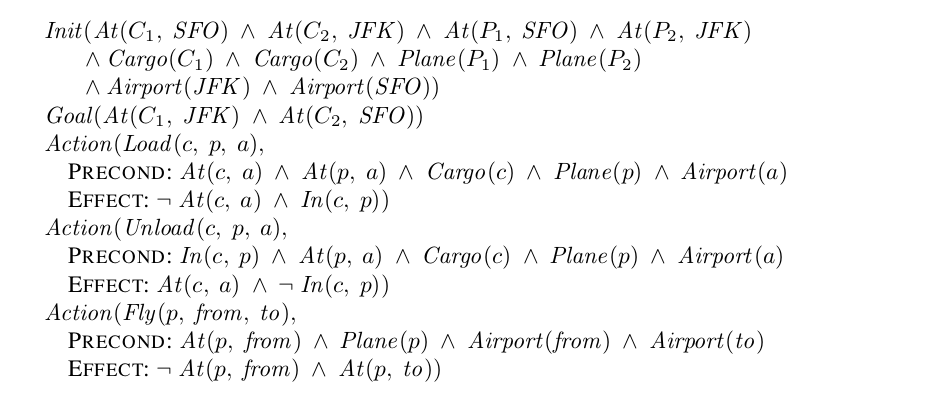
\includegraphics[scale=0.5]{cargo.png}
        \caption{Descrizione PDDL di un problema di pianificazione del trasporto di merci
        presente nel \textbf{Cap.10.1} del \textit{Russell e Norvig}.}
        \label{fig:birds}
    \end{figure}
    \subsubsection*{Descrizione generale del problema}
    \begin{itemize}
        \item \textbf{Dominio}, definito tramite assiomi
        \begin{itemize}
            \item Un insieme $C=\{c_i \ | \ $\texttt{Cargo($c_i$)}$\}$ di merci da trasportare,\\
            con $i=1 \dots m$, dove $|C|=m$.
            \item Un insieme $P=\{p_j \ | \ $\texttt{Plane($p_j$)}$\}$ di aerei,\\
            con $j=1 \dots n$, dove $|P|=n$.
            \item Un insieme $A=\{a_k \ | \ $\texttt{Airport($a_k$)}$\}$ di aeroporti,\\
            con $k=1 \dots l$, dove $|A|=l$.
        \end{itemize}
        \item \textbf{Fluenti}
        \begin{itemize}
            \item $At_{plane} = \{$\texttt{at(p$_i$,a$_k$)}$ \ | \ 1\leq i\leq n, 1 \leq k\leq l\}$,
            dove p$_i$ è l'aereo che si trova nell'areoporto a$_k$
            \item $At_{cargo}= \{$\texttt{at(c$_i$,a$_k$)}$  \ | \ 1\leq i\leq m, 1 \leq k\leq l\}$,
            dove c$_i$ è la merce che si trova nell'areoporto a$_k$
            \item $In= \{$\texttt{in(c$_i$,p$_k$)}$ \ | \ 1\leq i\leq m, 1 \leq k\leq n\}$,
            dove c$_i$ è la merce che si trova nell'aereo p$_k$
        \end{itemize}
        \item \textbf{Azioni}
        \begin{itemize}
            \item \texttt{fly(p$_i$,a$_{from}$,a$_{to}$)}, dove p$_i$ è l'aereo che vola dall'
            aeroporto a$_{from}$ all'areoporto a$_{to}$.
            \begin{itemize}
                \item \texttt{PRE}:
                \texttt{at(p$_i$,a$_{from}$) \& Plane(p$_i$) \& Airport(a$_{from}$)\\ \& Airport(a$_{to}$)}
                \item \texttt{POST}: \texttt{ not at(p$_i$,a$_{from}$) \& at(p$_i$,a$_{to}$)}
            \end{itemize}
            \item \texttt{load(c$_i$,p$_{j}$,a$_{k}$)}, dove c$_i$ è la merce che viene caricata
            sull'aereo p$_{j}$ nell'areoporto a$_{k}$.
            \begin{itemize}
                \item \texttt{PRE}:
                \texttt{at(p$_j$,a$_k$) \& at(c$_i$,a$_k$) \& Cargo(c$_i$) \& Plane(a$_j$)\\ \& Airport(a$_k$)}
                \item \texttt{POST}: \texttt{ not at(c$_i$,a$_k$) \& in(c$_i$,p$_j$)}
            \end{itemize}
            \item \texttt{unload(c$_i$,p$_{j}$,a$_{k}$)}, dove c$_i$ è la merce che viene scaricata
            dall'aereo p$_{j}$ nell'areoporto a$_{k}$.
            \begin{itemize}
                \item \texttt{PRE}:
                \texttt{ at(p$_j$,a$_k$) \& in(c$_i$,p$_j$) \& Cargo(c$_i$) \& Plane(a$_j$)\\ \& Airport(a$_k$)}
                \item \texttt{POST}: \texttt{ at(c$_i$,a$_k$) \& not in(c$_i$,p$_j$)}
            \end{itemize}
        \end{itemize}
        \item \textbf{Goal}
        \begin{itemize}
            \item $G \subseteq At_{cargo}$ è l'insieme dei fluenti che devono essere soddisfatti al fine
            di risolvere il problema di pianificazione. \textit{(Si noti che non è stato usato il simbolo di
            inclusione stretta, poichè è possibile definire un insieme di goal contenente tutti i possibili
            fluenti in $At_{cargo}$, naturalmente, a meno che vengano definiti domini triviali,
            non è possibile trovare una soluzione.)}
        \end{itemize}
    \end{itemize}

    \subsubsection*{Implementazioni}
    Si è scelto di risolvere il problema del trasporto in due modi diversi: il primo, \texttt{cargoSequential.cl},
    prevede la possibilità di eseguire, per ogni istante di tempo, una sola azione:
    \begin{center}
        \texttt{1\{occurs(A,S): action(A)\}1:- level(S).}
    \end{center}
    Questo vincolo implica che deve essere eseguita \textbf{almeno} e \textbf{al più} un'azione
    \texttt{A} nello stato \texttt{S} .
    Quindi, ad esempio, solo un aereo alla volta può caricare le merci al proprio interno,
    scaricarle o effettuare un volo tra due aeroporti.

    Naturalmente si tratta di un approccio poco realistico e non efficiente al problema, dal momento
    che ci si aspetterebbe che gli aerei siano indipendenti tra loro.
    Per questo motivo una seconda implementazione, \texttt{cargoParallel.cl} prevede la possibilità di
    effettuare più azioni nello istante di tempo
    \begin{center}
        \texttt{1\{occurs(A,S): action(A)\}:- level(S).}
    \end{center}
    L'assenza di un vincolo superiore significa che è possibile eseguire nello stesso stato \texttt{S}
    un numero arbitrario di azioni.

    Essendo i vincoli più rilevanti nella risoluzione del problema, si mette in evidenza che in entrambe
    le implementazioni:
    \begin{itemize}
        \item \textit{L'aereo può eseguire una sola azione alla volta}: non può caricare/scaricare due
        merci diverse nello stesso istante e naturalmente non può volare in una certa direzione e
        contemporaneamente effettuare altre azioni.
        \item \textit{Capienza illimitata}: il numero di merci che è possibile caricare su un aereo
        non è limitato.
        Si è scelto questo approccio perchè si tratta di un semplice rilassamento di vincoli rispetto al
        problema con \textit{capienza limitata}, da cui, quindi, non si discosta molto, pur potendo essere
        definito in modo più semplice.
        \item \textit{Eliminazione di azioni useless}: dal momento che l'azione
        \begin{center}
            \texttt{fly(Plane,From,To)}
        \end{center}
        non viola nessun vincolo quando \texttt{From=To}, ma si tratta di un'\textit{azione useless} (non è una
        \textit{no-op} perchè \texttt{Plane} effettua un volo), \texttt{fly} è stata definita come segue
        \begin{verbatim} action(fly(Plane,From,To)) :- plane(Plane), airport(From),
        airport(To), From!=To.
        \end{verbatim}
        imponendo come nuovo vincolo che non si possa mai effettuare un volo da e verso lo stesso areoporto.
    \end{itemize}

    \paragraph*{Il tempo\\}
    Si pone un limite al tempo di esecuzione del piano attraverso una congiunzione di vincoli relativi ai fluenti:
    \begin{center}
        \texttt{holds(Fluent,lastLev)}
    \end{center}
    dove \texttt{Fluent} è il fluente che si vuole rendere valido entro e non oltre il tempo \texttt{lastLev}.
    Inoltre gli effetti di ogni azione eseguita nel tempo \texttt{S} sono validi nel tempo \texttt{S+1}.

    \paragraph*{Cargo Sequential\\}
    Oltre alla definizione attraverso \texttt{ASP} delle precondizioni e postcondizioni è stato necessario
    definire due \textit{vincoli di persistenza}
    \begin{center}
        \texttt{holds(F,S+1):-holds(F,S),fluent(F),level(S),not -holds(F,S+1).}
    \end{center}
    Questo vincolo implica che se al tempo	\texttt{S} è il fluente \texttt{F} è valido, e non è possibile
    dimostrare che al tempo successivo (\texttt{S+1}) \texttt{F} non sia più valido
    (\texttt{not -holds(F,S+1)}), allora si può affermare che la validità di \texttt{F} persista anche
    al tempo \texttt{S+1}.

    Inoltre deve essere definito
    \begin{center}
        \texttt{-holds(F,S+1):- -holds(F,S),fluent(F),level(S),not holds(F,S+1).}
    \end{center}
    Questo secondo vincolo implica che, se al tempo	\texttt{S}, il fluente \texttt{F} non è valido,
    e non è possibile dimostrare che al tempo successivo (\texttt{S+1}) \texttt{F} sia valido
    (\texttt{not holds(F,S+1)}), allora si può affermare che la non validità di \texttt{F}
    persista anche al tempo \texttt{S+1}.

    Sono inoltre stati definiti dei vincoli globali tali che al tempo \texttt{S} non sia possibile che:
    \begin{enumerate}
        \item lo stesso aereo si trovi in due areoporti diversi. \label{itm:p_at}
        \begin{verbatim}
            :-  holds(at(Plane,Airport1),S),
            holds(at(Plane,Airport2),S),
            Airport1!=Airport2.
        \end{verbatim}
        \item la stessa merce si trovi in due areoporti diversi. \label{itm:c_at}
        \begin{verbatim}
            :-  holds(at(Cargo,Airport1),S),
            holds(at(Cargo,Airport2),S),
            Airport1!=Airport2.
        \end{verbatim}
        \item due aerei diversi contengano la stessa merce. \label{itm:c_in}
        \begin{verbatim}
            :-  holds(in(Cargo,Plane1),S),
            holds(in(Cargo,Plane2),S),
            Plane1!=Plane2.
        \end{verbatim}
    \end{enumerate}
    Si è optato per questo approccio in modo che si possa considerare come fallimento sia
    l'errata definizione dei fluenti validi al tempo \texttt{0}, ma anche la definizione inconsistente del goal.
    Per esempio, se si pone che al tempo \texttt{0} un aereo si trovi in due areoporti diversi, il fallimento è
    immediato, infatti nessuna soluzione è da prendere in considerazione.
    Vale lo stesso nel caso si ponga come goal che, ad esempio, una stessa merce si trovi in due areoporti diversi.


    \paragraph*{Cargo Parallel\\}
    Dal momento che il numero di azioni eseguibili in un singolo stato non è limitato a 1, è necessario
    definire vincoli globali in modo che tale rilassamento del problema non crei inconsistenze.
    Nonostante sia intuitivo pensare di rispettare tale regola tramite il seguente vincolo:
    \begin{center}
        \texttt{:- occurs(Action1,S), occurs(Action2,S), Action1!=Action2.}
    \end{center}
    In realtà questo vincolo elimina il rilassamento voluto, dal momento che non è possibile eseguire
    più di un azione alla volta, anche rispetto ad aerei diversi.
    Quindi è necessario definire i vincoli globali facendo riferimento in modo specifico agli aerei e alle merci:
    non è possibile che al tempo \texttt{S}
    \begin{enumerate}

        \item lo stesso aereo carichi/scarichi due merci diverse.
        \begin{verbatim}
            :-  occurs(load/unload(Cargo1,Plane,_),S),
            occurs(load/unload(Cargo2,Plane,_),S),
            Cargo1!=Cargo2.
        \end{verbatim}
        \item lo stesso aereo effettui un qualche volo e carichi una qualche merce.
        \begin{verbatim}
            :-  occurs(fly(Plane,_,_),S),
            occurs(load(_,Plane,_),S).
        \end{verbatim}
        \item lo stesso aereo effettui un qualche volo e scarichi una qualche merce.
        \begin{verbatim}
            :-  occurs(fly(Plane,_,_),S),
            occurs(unload(_,Plane,_),S).
        \end{verbatim}
        \item lo stesso aereo scarichi una qualche merce e carichi una qualche merce.
        \begin{verbatim}
            :-  occurs(unload(_,Plane,_),S),
            occurs(load(_,Plane,_),S).
        \end{verbatim}
    \end{enumerate}
    Si è potuto omettere alcuni elementi sfruttando le proprietà del carattere "\texttt{\_}",
    che ha il significato sintattico di poter essere sostituito con qualsiasi elemento che rispetti
    il pattern matching: non è necessario in questo caso rendere espliciti i vincoli relativi
    alle precondizioni e postcondizioni, poichè devono essere già rispettati.

    Nonostante le regole~\ref{itm:p_at},~\ref{itm:c_at} e~\ref{itm:c_in}, nel caso \textit{parallelo}
    possano essere equivalentemente sostituite da regole che considerino le azioni e non i fluenti,
    si è preferito mantenere lo stesso approccio del caso precedente.


    \subsubsection*{Soluzione e fallimento}
    Per imporre che sia soddisfatta la validità di un insieme di fluenti si definisce, innanzitutto, la regola
    \begin{center}
        \texttt{goal :- subgoal\_c$_1$, \dots, subgoal\_c$_n$}
    \end{center}
    dove \texttt{subgoal\_c$_i$} è della forma \texttt{holds(F$_i$,S$_i$)}, dove \texttt{F$_i$} \texttt{ed S$_i$}
    sono rispettivamente il fluente e il tempo del sottogoal dell'\textit{i}-esima merce \texttt{c$_i$}.

    Poi si pone il vincolo
    \begin{center}
        \texttt{:- not goal}
    \end{center}
    Se non è possibile rendere valido \texttt{goal} in almeno un modello il problema non è risolvibile.

    Tutte le possibili soluzioni al problema sono date dai possibili modelli che rendono valido \texttt{goal}.


    \subsubsection*{Esempi}
    Sono presi in considerazione 6 possibili scenari, con 3 tipi di dominio diversi (\textit{piccolo, medio, grande}),
    e 2 difficoltà diverse per ogni dominio (\textit{facile, difficile}).

    \begin{itemize}
        \item \textbf{Dominio}

        \begin{tabular}{|c | c| c |c |}
            \hline
            &$|P|$&$|C|$&$|A|$\\
            \hline
            Piccolo &1&2&3\\
            \hline
            Medio   &2&4&5\\
            \hline
            Grande  &2&8&9\\
            \hline
        \end{tabular}
        \item \textbf{Difficoltà}
        Tutte le merci si trovano in un areoporto diverso da quello di destinazione.
        Questo perchè altrimenti si avrebbero alcune configurazioni triviali per alcune merci: la soluzione per il
        sottogoal in questione è una lista vuota di azioni.
        \begin{itemize}

            \item Facile
            \begin{enumerate}
                \item Ogni aereo si trova al tempo \texttt{0} in un areoporto con almeno una merce.
                \item Più merci possono trovarsi nello stesso areoporto al tempo \texttt{0}. \label{itm:same_airport}
                \item Le merci hanno la stessa destinazione.
            \end{enumerate}
            (il punto \ref{itm:same_airport} è definito in questo modo perchè non si è voluto presentare problemi
            banali, come quello in cui tutte le merci si trovano nello stesso areoporto e hanno la stessa destinazione)\\
            \item Difficile
            \begin{enumerate}
                \item Ogni aereo si trova al tempo \texttt{0} in un areoporto senza merci.
                \item Tutte le merci si trovano in areoporti diversi al tempo \texttt{0}.
                \item Tutte le merci hanno una destinazione diversa.
            \end{enumerate}
        \end{itemize}
    \end{itemize}

    Le seguenti tabelle presentano il numero minimo di passi per ogni configurazione, rispettivamente, per la soluzione
    sequenziale (un'azione alla volta) e per quella parallela (più azioni alla volta per aerei diversi).
    Come si può notare per il dominio piccolo, essendo presente un solo aereo, le due soluzioni sono equivalenti.
    \begin{center}

        \begin{tabular}{l c c c c c c}
            \toprule % Top horizontal line
            &\multicolumn{6}{c}{Numero minimo di passi} \\
            \cmidrule(l){2-7}
            & \multicolumn{2}{c}{Piccolo} & \multicolumn{2}{c}{Medio} & \multicolumn{2}{c}{Grande} \\
            \cmidrule(l){2-7}
            Strategia & Facile & Difficile & Facile & Difficile & Facile & Difficile\\
            \midrule
            Sequenziale &5  &6  &10 &12 & 20    & 25\\ % Content row 1
            Parallelo   &5  &6  &5  &6  & 10    & 12\\ % Content row 2

            \bottomrule
        \end{tabular}
    \end{center}

    \begin{center}
        \begin{tabular}{l c c c c c c}
            \toprule % Top horizontal line
            &\multicolumn{6}{c}{Tempo di esecuzione (in secondi)} \\
            \cmidrule(l){2-7}
            & \multicolumn{2}{c}{Piccolo} & \multicolumn{2}{c}{Medio} & \multicolumn{2}{c}{Grande} \\
            \cmidrule(l){2-7}
            Strategia & Facile & Difficile & Facile & Difficile & Facile & Difficile\\
            \midrule
            Sequenziale & 0.008 & 0.008 & 0.081 & 0.081 & 2428.557  & 2727.133 \\ % Content row 1
            Parallelo   & 0.008 & 0.008 & 0.041 & 0.041 & 3.026     & 48.202\\ % Content row 2

            \bottomrule
        \end{tabular}
    \end{center}
    Quando il problema non è soddisfacibile è possibile che, per domini molto grandi, il tempo richiesto
    per ottenere il risultato negativo sia troppo elevato, quindi interrompendo l'esecuzione non è possibile dimostrare
    che il problema non sia risolvibile con un dato numero di passi.
    Nel caso della procedura sequenziale per il dominio grande difficile, l'esecuzione con 24 passi è stata fermata
    dopo 21223.197 secondi, cioè quasi 6 ore.
    Vista la proporzione tra la difficoltà facile e difficile della strategia parallela si potrebbe ipoteticamente
    assumere che il numero minimo di passi per la prima strategia nel caso \textit{dominio grande difficile} non sia 25,
    ma 24.
    Il problema è che, come sopra detto, la durata dell'esecuzione sarebbe troppo elevata: supponendo che la proporzione
    sia approssimativamente affidabile, sarebbe necessario attendere più di $38.400$, cioè quasi 11 ore.
    \newpage
    \subsubsection*{Guida all'esecuzione}
    I file sono i seguenti
    \begin{itemize}
        \item \textbf{Procedure}
        \begin{itemize}
            \item \texttt{cargoSequential.cl}: procedura sequenziale
            \item \texttt{cargoParallel.cl}: procedura parallela
        \end{itemize}
        \item \textbf{Dominio}
        \begin{itemize}
            \item \texttt{smallDomain.cl}: dominio piccolo (|P|=1, |C|=2, |A|=3)
            \item \texttt{mediumDomain.cl}: dominio medio (|P|=2, |C|=4, |A|=5)
            \item \texttt{bigDomain.cl}: dominio grande (|P|=2, |C|=8, |A|=9)
        \end{itemize}
        \item \textbf{Difficoltà}
        \begin{itemize}
            \item \texttt{easy<nome\_dominio>.cl}: una configurazione facile per ogni dominio
            \item \texttt{hard<nome\_dominio>.cl}: una configurazione difficile per ogni dominio
        \end{itemize}
    \end{itemize}
    Per avviare l'esecuzione è necessario esplicitare i seguenti parametri:
    \begin{verbatim}
        clingo <procedura> <dominio> <difficoltà>
    \end{verbatim}
    Il numero di passi massimo di esecuzione è definito nei file \texttt{<difficoltà>}.
    \newpage
    \noindent

    \section*{Appendice}
    \subsection*{Scenari dei test degli algoritmi Prolog}
    \paragraph*{Labirinto\\}
    In rosso sono indicate le posizioni difficili, in verde quelle facili;
    P e A indicano le caselle di 	partenza ed arrivo.\\\\
    \textit{Labirinto 10x10}
    \begin{center}
        \begin{tikzpicture}[scale=1]

            \begin{scope}[thick,local bounding box=name]
                \ColorCellsBlackTen{
                5/2,5/3,5/4,5/5,5/6,5/7,1/7,2/7,3/7,4/7,
                7/4,8/4,9/4,10/4,7/5,7/6,7/7,7/8}{10}{1cm}
                \ColorCellsTen{2/4/red,9/7/red,4/6/green,3/8/green}{10}{1cm}
                \draw (0, 0) grid (10, 10);
            \end{scope}
            \TextColumnTen{2/4/{P}}{10}{1cm}
            \TextColumnTen{4/6/{P}}{10}{1cm}
            \TextColumnTen{9/7/{A}}{10}{1cm}
            \TextColumnTen{3/8/{A}}{10}{1cm}

        \end{tikzpicture}
    \end{center}
    \newpage
    \noindent\textit{Labirinto 20x20}
    \begin{center}
        \begin{tikzpicture}[scale=0.75]

            \begin{scope}[thick,local bounding box=name]
                \ColorCellsBlackTen{
                1/15,2/15,3/15,4/15,5/15,6/15,7/15,8/15,9/15,
                6/13,7/13,8/13,9/13,10/13,11/13,12/13,13/13,14/13,15/13,
                15/7,15/8,15/9,15/10,15/11,15/12}{20}{0.75cm}
                \ColorCellsTen{10/10/red,20/20/red,14/12/green,16/14/green}{20}{0.75cm}
                \draw (0, 0) grid (20, 20);
            \end{scope}
            \TextColumnTen{14/12/{P}}{20}{0.75cm}
            \TextColumnTen{10/10/{P}}{20}{0.75cm}
            \TextColumnTen{16/14/{A}}{20}{0.75cm}
            \TextColumnTen{20/20/{A}}{20}{0.75cm}

        \end{tikzpicture}
    \end{center}
    \newpage
    \paragraph*{Gioco delle tessere\\\\}
    \textit{Gioco dell'8 facile}
    \begin{center}
        \begin{tikzpicture}[scale=1]

            \begin{scope}[thick,local bounding box=name]
            \end{scope}
            \TextColumnTen{1/1/{3}}{3}{1cm}
            \TextColumnTen{1/2/{6}}{3}{1cm}
            \TextColumnTen{1/3/{2}}{3}{1cm}
            \TextColumnTen{2/1/{4}}{3}{1cm}
            \TextColumnTen{2/2/{}}{3}{1cm}
            \TextColumnTen{2/3/{7}}{3}{1cm}
            \TextColumnTen{3/1/{1}}{3}{1cm}
            \TextColumnTen{3/2/{8}}{3}{1cm}
            \TextColumnTen{3/3/{5}}{3}{1cm}
            \draw (0, 0) grid (3, 3);

        \end{tikzpicture}
    \end{center}
    \textit{Gioco dell'8 difficile}
    \begin{center}
        \begin{tikzpicture}[scale=1]

            \begin{scope}[thick,local bounding box=name]
            \end{scope}
            \TextColumnTen{1/1/{}}{3}{1cm}
            \TextColumnTen{1/2/{6}}{3}{1cm}
            \TextColumnTen{1/3/{2}}{3}{1cm}
            \TextColumnTen{2/1/{3}}{3}{1cm}
            \TextColumnTen{2/2/{8}}{3}{1cm}
            \TextColumnTen{2/3/{5}}{3}{1cm}
            \TextColumnTen{3/1/{7}}{3}{1cm}
            \TextColumnTen{3/2/{1}}{3}{1cm}
            \TextColumnTen{3/3/{4}}{3}{1cm}
            \draw (0, 0) grid (3, 3);
        \end{tikzpicture}
    \end{center}
    \textit{Gioco dell'15 facile}
    \begin{center}
        \begin{tikzpicture}[scale=1]

            \begin{scope}[thick,local bounding box=name]
            \end{scope}
            \TextColumnTen{1/1/{7}}{4}{1cm}
            \TextColumnTen{1/2/{5}}{4}{1cm}
            \TextColumnTen{1/3/{6}}{4}{1cm}
            \TextColumnTen{1/4/{9}}{4}{1cm}
            \TextColumnTen{2/1/{2}}{4}{1cm}
            \TextColumnTen{2/2/{10}}{4}{1cm}
            \TextColumnTen{2/3/{3}}{4}{1cm}
            \TextColumnTen{2/4/{13}}{4}{1cm}
            \TextColumnTen{3/1/{1}}{4}{1cm}
            \TextColumnTen{3/2/{4}}{4}{1cm}
            \TextColumnTen{3/3/{}}{4}{1cm}
            \TextColumnTen{3/4/{14}}{4}{1cm}
            \TextColumnTen{4/1/{8}}{4}{1cm}
            \TextColumnTen{4/2/{12}}{4}{1cm}
            \TextColumnTen{4/3/{15}}{4}{1cm}
            \TextColumnTen{4/4/{11}}{4}{1cm}
            \draw (0, 0) grid (4, 4);
        \end{tikzpicture}
    \end{center}
    \textit{Gioco dell'15 difficile}
    \begin{center}
        \begin{tikzpicture}[scale=1]

            \begin{scope}[thick,local bounding box=name]
            \end{scope}
            \TextColumnTen{1/1/{15}}{4}{1cm}
            \TextColumnTen{1/2/{6}}{4}{1cm}
            \TextColumnTen{1/3/{9}}{4}{1cm}
            \TextColumnTen{1/4/{13}}{4}{1cm}
            \TextColumnTen{2/1/{5}}{4}{1cm}
            \TextColumnTen{2/2/{8}}{4}{1cm}
            \TextColumnTen{2/3/{12}}{4}{1cm}
            \TextColumnTen{2/4/{7}}{4}{1cm}
            \TextColumnTen{3/1/{3}}{4}{1cm}
            \TextColumnTen{3/2/{2}}{4}{1cm}
            \TextColumnTen{3/3/{}}{4}{1cm}
            \TextColumnTen{3/4/{10}}{4}{1cm}
            \TextColumnTen{4/1/{11}}{4}{1cm}
            \TextColumnTen{4/2/{1}}{4}{1cm}
            \TextColumnTen{4/3/{4}}{4}{1cm}
            \TextColumnTen{4/4/{14}}{4}{1cm}
            \draw (0, 0) grid (4, 4);
        \end{tikzpicture}
    \end{center}


    \newpage
    \subsection*{Configurazioni problema del trasporto}
    \paragraph*{Dominio Piccolo (|P|=1, |C|=2, |A|=3)\\\\}
    \noindent \textit{Facile\\}
    \begin{minipage}{0.45\textwidth}
        \begin{center}
            \captionof{table}*{START}
            \begin{tabular}{|c | c| c |}
                \hline
                A1&A2&A3\\
                \hline
                \textbf{C1} P1&\textbf{C2}&\\
                \hline
            \end{tabular}
        \end{center}
    \end{minipage}%
    \begin{minipage}{0.45\textwidth}
        \begin{center}
            \captionof{table}*{GOAL}
            \begin{tabular}{|c | c| c |}
                \hline
                A1&A2&A3\\
                \hline
                \textbf{C2}&\textbf{C1}&\\
                \hline
            \end{tabular}
        \end{center}
    \end{minipage}%

    \noindent \textit{ \\\\ Difficile\\}
    \begin{minipage}{0.45\textwidth}
        \begin{center}
            \captionof{table}*{START}
            \begin{tabular}{|c | c| c |}
                \hline
                A1&A2&A3\\
                \hline
                \textbf{C1} &\textbf{C2}&P1\\
                \hline
            \end{tabular}
        \end{center}
    \end{minipage}%
    \begin{minipage}{0.45\textwidth}

        \begin{center}
            \captionof{table}*{GOAL}
            \begin{tabular}{|c | c| c |}
                \hline
                A1&A2&A3\\
                \hline
                \textbf{C2}&\textbf{C1}&\\
                \hline
            \end{tabular}

        \end{center}
    \end{minipage}
    \paragraph*{Dominio Medio  (|P|=2, |C|=4, |A|=5)\\\\}

    \noindent \textit{Facile\\}
    \begin{minipage}{0.45\textwidth}

        \begin{center}
            \captionof{table}*{START}
            \begin{tabular}{|c | c| c | c | c |}
                \hline
                A1&A2&A3&A4&A5\\
                \hline
                \textbf{C1} P1&\textbf{C2 C4} P2&\textbf{C3}&&\\
                \hline
            \end{tabular}

        \end{center}
    \end{minipage}
    \begin{minipage}{0.45\textwidth}

        \begin{center}
            \captionof{table}*{GOAL}
            \begin{tabular}{|c | c| c | c | c |}
                \hline
                A1&A2&A3&A4&A5\\
                \hline
                \textbf{C3 C4}&\textbf{C1}&\textbf{C3}&&\\
                \hline
            \end{tabular}

        \end{center}
    \end{minipage}

    \noindent \textit{ \\\\ Difficile\\}
    \begin{minipage}{0.45\textwidth}

        \begin{center}
            \captionof{table}*{START}
            \begin{tabular}{|c | c| c | c | c |}
                \hline
                A1&A2&A3&A4&A5\\
                \hline
                \textbf{C1}&\textbf{C2}&\textbf{C3}&\textbf{C4}&P1 P2\\
                \hline
            \end{tabular}

        \end{center}
    \end{minipage}
    \begin{minipage}{0.45\textwidth}

        \begin{center}
            \captionof{table}*{GOAL}
            \begin{tabular}{|c | c| c | c | c |}
                \hline
                A1&A2&A3&A4&A5\\
                \hline
                \textbf{C4}&\textbf{C1}&\textbf{C2}&\textbf{C3}&\\
                \hline
            \end{tabular}

        \end{center}
    \end{minipage}


    \paragraph*{Dominio Grande  (|P|=2, |C|=8, |A|=9)\\\\}

    \noindent \textit{Facile}

    \begin{center}
        \captionof{table}*{START}
        \begin{tabular}{|c | c| c | c | c | c | c | c |c |}
            \hline
            A1&A2&A3&A4&A5&A6&A7&A8&A9\\
            \hline
            \textbf{C1 C2 C3} P1 &\textbf{C4 C5 C6} P2&\textbf{C7 C8}&&&&&&\\
            \hline
        \end{tabular}

    \end{center}
    \begin{center}
        \captionof{table}*{GOAL}
        \begin{tabular}{|c | c| c | c | c | c | c | c |c |}
            \hline
            A1&A2&A3&A4&A5&A6&A7&A8&A9\\
            \hline
            \textbf{C4 C7}&\textbf{C1 C8}&\textbf{C2 C5}&\textbf{C3 C6}&&&&&\\
            \hline
        \end{tabular}

    \end{center}

    \noindent \textit{Difficile}

    \begin{center}
        \captionof{table}*{START}
        \begin{tabular}{|c | c| c | c | c | c | c | c |c |}
            \hline
            A1&A2&A3&A4&A5&A6&A7&A8&A9\\
            \hline
            \textbf{C1}  &\textbf{C2} &\textbf{C3}&\textbf{C4}&\textbf{C5}
            &\textbf{C6}&\textbf{C7}&\textbf{C8}&P1 P2\\
            \hline
        \end{tabular}

    \end{center}
    \begin{center}
        \captionof{table}*{GOAL}
        \begin{tabular}{|c | c| c | c | c | c | c | c |c |}
            \hline
            A1&A2&A3&A4&A5&A6&A7&A8&A9\\
            \hline
            \textbf{C8}  &\textbf{C1} &\textbf{C2}&\textbf{C3}&\textbf{C4}
            &\textbf{C5}&\textbf{C6}&\textbf{C7}&\\
            \hline
        \end{tabular}

    \end{center}
\end{document}